
\documentclass[preprint,12pt]{elsarticle}

\usepackage[spanish]{babel}
\usepackage{amssymb}
\usepackage{graphicx}
\usepackage{lineno}
\usepackage[utf8]{inputenc}
\usepackage{url}
\usepackage{natbib}

\begin{document}
	
	\begin{frontmatter}

		\title{\huge SQL:2003 is the ISO/IEC 9075:2003 standard of 2003}
		
		\author{José Edilberto Pastor Mendoza               (2016055237)}
		
		\address{Tacna, Perú}
		
		\begin{abstract}
			%% Text of abstract
ISO/IEC 9075 defines the SQL language. The scope of the SQL language is the definition of data structure and the operations on data stored in that structure. Parts 1, 2 and 11 encompass the minimum requirements of the language. Other parts define extensions.

ISO/IEC 9075-1:2003 describes the conceptual framework used in other parts of ISO/IEC 9075 to specify the grammar of SQL and the result of processing statements in that language by an SQL-implementation.


		\end{abstract}
\end{frontmatter}
%%
	%% Start line numbering here if you want
	%%
	%\linenumbers
	
	%% main text
	\section{Resumen}

ISO / IEC 9075 define el lenguaje SQL. El alcance del lenguaje SQL es la definición de la estructura de datos y las operaciones sobre los datos almacenados en esa estructura. Las partes 1, 2 y 11 abarcan los requisitos mínimos del idioma. Otras partes definen extensiones.


	%%
	%% Start line numbering here if you want
	%%
	%\linenumbers
	
	%% main text
\section{Introduccion}
SQL: 2003 realiza revisiones a todas las partes de SQL: 1999
y agrega una nueva parte Además,hay
alguna ligera reorganización de las partes heredadas de
SQL: 1999. Una parte sustancial de SQL: Parte 2 de 1999:
SQL / Foundation que trató con la información
Esquema y definición El esquema se divide en su
Parte propia, Parte 11: SQL / Esquemas en SQL: 2003.
SQL: Parte 5 de 1999: SQL / Bindings ha sido
eliminado en SQL: 2003 al fusionar todo el material
contenido en esa parte en SQL: 2003 Parte 2:
SQL / Foundation.
En este artículo, nos enfocamos en lo siguiente
\begin{itemize}
		\item Beneficios de SQL 
		\item Concepto de SQL
	\end{itemize}

	%%
	%% Start line numbering here if you want
	%%
	%\linenumbers
	
	%% main text

%\section{Objetivo}
%		\begin{itemize}
%		\item Objetivo 1:
%		\item Objetivo 2: 
%		\item Objetivo 3: 
%
%	\end{itemize}

	%%
	%% Start line numbering here if you want
	%%
	%\linenumbers
	
	%% main text

\section{Marco Teorico}
	
\subsection{SQL}	

El SQL es el lenguaje estándar ANSI/ISO de definición, manipulación y control
de bases de datos relacionales. Es un lenguaje declarativo: sólo hay que indicar
qué se quiere hacer. En cambio, en los lenguajes procedimentales es necesario
especificar cómo hay que hacer cualquier acción sobre la base de datos. El SQL
es un lenguaje muy parecido al lenguaje natural; concretamente, se parece al
inglés, y es muy expresivo. Por estas razones, y como lenguaje estándar, el SQL
es un lenguaje con el que se puede acceder a todos los sistemas relacionales
comerciales.

%\begin{itemize}

%\item Representa una foto abstracta de la organización del negocio por diferentes áreas.
%\item Sus datos están muy estructurados y organizados.
%\item No tiene datos cuyo uso no haya sido definido previamente.

%\end{itemize}

\begin{figure}[htb]
				\begin{center}
					
\includegraphics[width=15cm]{./IMAGENES/sql}
				\end{center}
			\end{figure}

\subsection{PRINCIPALES VENTAJAS DE SQL}	
\begin{figure}[htb]
				\begin{center}
					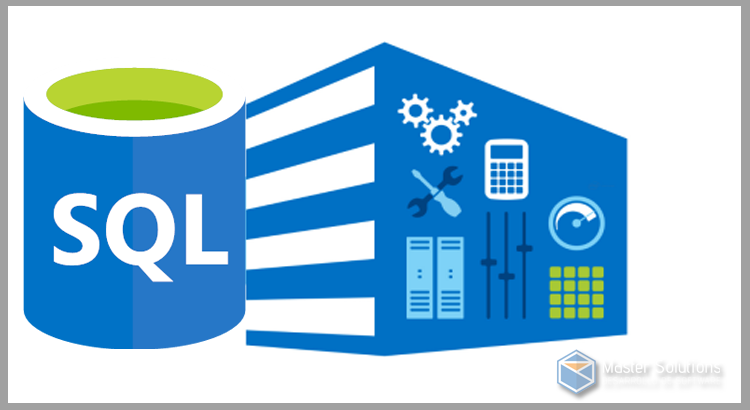
\includegraphics[width=15cm]{./IMAGENES/sqldos}
				\end{center}
			\end{figure}
Estas son las principales ventajas que se pueden encontrar en el lenguaje SQL:
\begin{itemize}

\item Es un sistema de gestión de base de datos.
\item Es útil para manejar y obtener datos de la red de redes.
\item Nos permite olvidarnos de los ficheros que forman la base de datos.
\item SQL permite administrar permisos a todo. También  permite que  alguien conecte su SQLO al nuestro pero sin embargo podemos decirle que no puede ver esta base de datos pero otro si.
\end{itemize}

\subsection{DESVENTAJAS DE SQL}	

\begin{itemize}

\item Utiliza mucho la memoria RAM  para las instalaciones y utilización de software.
\item La relación, calidad y el precio esta muy debajo comparado con oracle.
\end{itemize}
Las empresas que utilizan SQL son fundamentalmente aquellas que manejan grandes volúmenes de datos relativos a clientes, compras, marketing, transacciones, operaciones. como lo son las empresas de telecomunicaciones, transporte, Turismo, fabricación de bienes de consumo masivo etc.

\subsection{ISO/IEC 9075}

Norma ISO / IEC 9075: "Tecnología de la información - Lenguajes de base de datos - SQL", que describe el lenguaje de consulta estructurado.

describe el marco conceptual utilizado en otras partes de ISO / IEC 9075 para especificar la gramática de SQL y el resultado del procesamiento de declaraciones en ese lenguaje mediante una implementación de SQL.


%\begin{itemize}
	
%\item Contiene todos los datos de las fuentes originales, sin rechazar ningún tipo de dato.
%\item Los datos se almacenan sin transformar o apenas transformados.
%\item Los datos se transforman y se aplica un esquema sólo para satisfacer las necesidades %de análisis.

%\end{itemize}

%\begin{figure}[htb]
%				\begin{center}
%					\includegraphics[width=15cm]{./IMAGENES/fiorella2}
%				\end{center}
%			\end{figure}


%\begin{figure}[htb]
%				\begin{center}
%					\includegraphics[width=15cm]{./IMAGENES/fiorella3}
%				\end{center}
%			\end{figure}
%En definitiva es importante saber que aun siendo ambos conceptos, Data Warehouse y Data Lake, repositorios de información, un Data Lake no es una nueva versión 2.0 de un Data Warehouse ni su remplazo.

%De hecho, se pueden complementar muy bien, diseñando una arquitectura de datos moderna, que permita seguir a las organizaciones aprovechando sus inversiones en su Data Warehouse, mientras que empiezan a recoger en su Data Lake, todos los datos que han sido ignorados o desechados anteriormente.

%\subsection{PRINCIPALES BENEFICIOS DE UN DATA LAKE}	


%Un Data Lake tiene muchas ventajas. Las más destacables son estas:

%\begin{itemize}



\subsection{SQL:2003 ONTOLOGY}
	
Entre los diferentes idiomas presentes en el
DBMS más temprano, SQL se ha impuesto como un "de
iure "y el estándar de base de datos" de facto ".
Recientemente, la última versión del estándar ha sido
publicado, SQL: 2003 (ISO / IEC 9075, 2003) que
realiza revisiones a todas las partes de SQL: 1999 y
incluye algunos temas nuevos (Eisenberg et al., 2004).
El hecho de tener un estándar es fundamental.
Sin embargo, a veces los estándares son difíciles de
entender y es difícil extraer todo el
información contenida Suele suceder que
los estándares no están libres de inconsistencias debido a
gran cantidad de información que intentan cubrir. En
en ese caso, la mayoría de las ventajas derivadas de la
eliminación de un estándar desaparecer.
Para evitar la mayoría de estos problemas, el
El estándar puede complementarse con su ontología. En
de tal manera la ontología ayuda a encontrar el
información y detección de inconsistencias que es
esencial para definir las métricas basadas en el
conceptos de la norma.
Una ontología es una especificación de un
conceptualización Esto significa que, a través del
definición de una ontología, tratamos de formalizar y
recuperar el conocimiento de un dominio dado.
Desarrollamos una ontología para el SQL: 2003.
Para hacerlo, hemos trabajado principalmente con el
información de la parte 1 (Marco) pero básicamente
con el de la parte 2 (Fundación) de la norma.
Por otro lado, también rediseñamos la Parte 11
(Esquema de información y definición) considerando
esos esquemas como metamodelos del SQL: 2003
que representan en sus tablas todos los conceptos de la
idioma.


\section{Apreciación}
\begin{itemize}
\item Apreciación : \\

SQL es un lenguaje declarativo estándar internacional de comunicación dentro de las bases de datos que nos permite a todos el acceso y manipulación de datos en una base de datos, y además se puede integrar a lenguajes de programación, por ejemplo ASP o PHP, y en combinación con cualquier base de datos específica, por ejemplo MySQL, SQL Server, MS Access, entre otras

\end{itemize}
\section{Conclusion}
\begin{itemize}
\item Conclusion : \\

las habilidades en SQL para trabajar en programas y bases de datos se han hecho más necesarias, valiosas y recompensadas. Las empresas están buscando la ayuda de personas que conocen SQL. Ellos saben el valor que alguien experto en SQL aporta a su empresa y buscan emplear a estas personas.

En el futuro las compañías necesitarán cada vez más trabajadores con experiencia en el acceso y análisis de información, y SQL te posibilitará alcanzar esos conocimientos.


\end{itemize}
%%
	
	%%
	%\linenumbers
	
	%% main text

	
	\newpage
	
	\bibliographystyle{apalike} 	%ESTILO
	\bibliography{BIBLIOGRAFIA}	 
\citep{referencia01}  
\citep{referencia02}  
\citep{referencia03}  
\citep{referencia04}  
\citep{referencia05} 
%ARCHIVO .bib
	
	%% The Appendices part is started with the command \appendix;
	%% appendix sections are then done as normal sections
	%% \appendix
	
	%% \section{}
	%% \label{}
	
	%% References
	%%
	%% Following citation commands can be used in the body text:
	%% Usage of \cite is as follows:
	%%   \cite{key}          ==>>  [#]
	%%   \cite[chap. 2]{key} ==>>  [#, chap. 2]
	%%   \citet{key}         ==>>  Author [#]
	
	%% References with bibTeX database:
	
	
	%% Authors are advised to submit their bibtex database files. They are
	%% requested to list a bibtex style file in the manuscript if they do
	%% not want to use model1-num-names.bst.
	
	%% References without bibTeX database:
	
	% \begin{thebibliography}{00}
	
	%% \bibitem must have the following form:
	%%   \bibitem{key}...
	%%
	
	% \bibitem{}
	
	% \end{thebibliography}
	
\end{document}

%%
%% End of file `elsarticle-template-1-num.tex'.
